\section{Instructions de mission}\label{instructions-de-mission}

\subsection{Iceberg}\label{iceberg}

Dans le cadre de votre mission, vous serez envoyé au Pôle Sud, sur un
des icebergs où nos services de renseignements ont indiqué que les
premiers repérages aliens auront lieu. L'iceberg est représenté par une
grille carrée de 25 cases de côté.

\begin{figure}[!h]
    \centering
    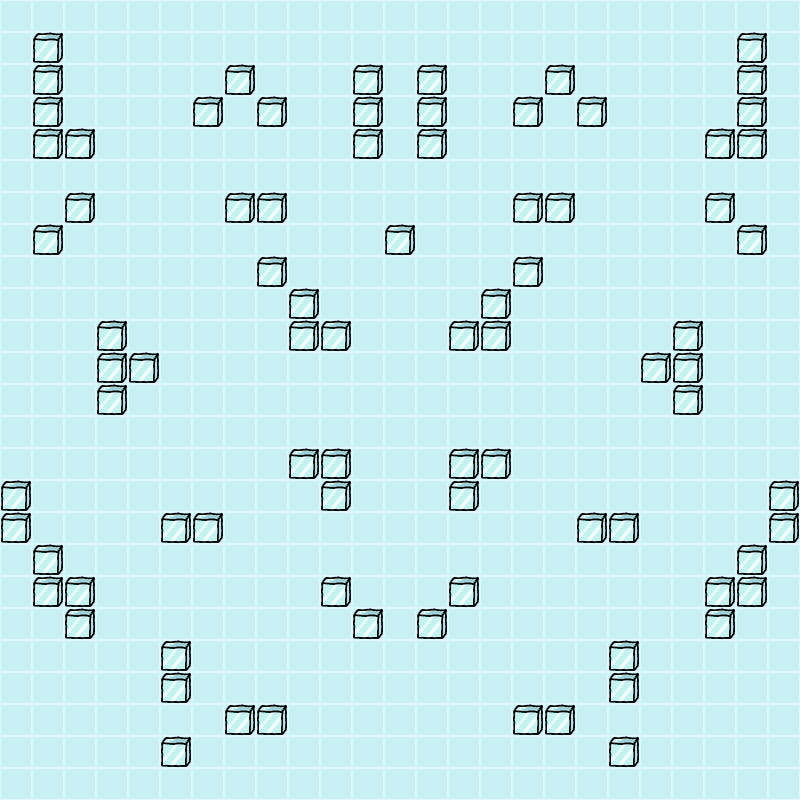
\includegraphics[width=9cm]{img/map.png}
    \caption*{Un exemple d'iceberg.}
\end{figure}

Une position sur l'iceberg est notée à l'aide d'un couple $(ligne,
colonne)$, où $0 \leq ligne, colonne < 25$.

\subsubsection{Cases}\label{cases}

Chaque case de l'iceberg est soit libre, soit un mur de glace. Les murs
sont des obstacles et bloquent tout déplacement sur la case.

Une case libre peut contenir un alien ainsi qu'un agent. À noter qu'il
est impossible d'avoir plusieurs agents ou plusieurs aliens sur une même
case.

\subsubsection{Agents}\label{agents}

Les deux recrues PiB ont à leur disposition quatre agents, numérotés de
0 à 3. Ces derniers sont considérés comme des obstacles, et bloquent
donc tout déplacement sur la case.

\begin{figure}[!h]
    \centering
    
\includegraphics[width=1.5cm]{img/penguin}
    \caption*{Un agent PiB.}
\end{figure}

\subsubsection{Aliens}\label{aliens}

Des aliens débarqueront sur l'iceberg à des positions précises de la
carte, pendant un certain nombre de tours afin d'accomplir leur mission
de reconnaissance, avant de repartir sur leur planète d'origine. De
plus, les aliens n'envahissent jamais plusieurs fois au même endroit sur
l'iceberg.

\begin{figure}[!h]
    \centering
    
\includegraphics[width=1.5cm]{img/alien}
    \caption*{Un alien menaçant.}
\end{figure}

Pour capturer un alien, un agent doit être sur la case pendant au moins
3 tours. L'alien capturé disparaît de l'iceberg, et des échantillons
d'analyse sont envoyés instantanément au QG des PiB, l'agent peut donc
continuer sa mission. Si l'agent quitte la case, ne serait-ce qu'un
instant (en se déplaçant ou alors en étant poussé par un agent), la
capture devra reprendre de \textbf{zéro}.

\begin{figure}[!h]
    \centering
    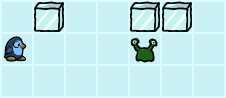
\includegraphics[width=4.5cm]{img/alien_capture1}
    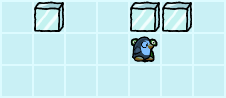
\includegraphics[width=4.5cm]{img/alien_capture2}
    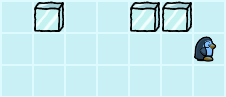
\includegraphics[width=4.5cm]{img/alien_capture3}
    \vspace{-0.3cm}
    \caption*{(3 tours)}
    \caption*{Un agent qui capture un alien, puis continue sa mission.}
\end{figure}

Les aliens ne sont pas assez habitués à la glace pour se déplacer sur
l'iceberg. Ils se contenteront donc pour leur mission de repérage de
rester fixes par rapport à leurs lieux d'invasion. En revanche, les
aliens ne sont pas des obstacles : faisant des efforts admirables pour
éviter les agents - contrairement aux murs, qui sont davantage
récalcitrants - ils se contorsionneront et esquiveront de leur mieux :
ils ne bloquent donc pas le déplacement des agents.

\begin{figure}[!h]
    \centering
    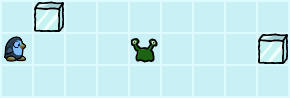
\includegraphics[width=5cm]{img/alien_not_obstacle1}
    \hspace{0.5cm}
    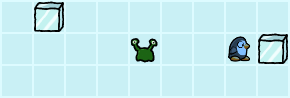
\includegraphics[width=5cm]{img/alien_not_obstacle2}
    \caption*{Les aliens ne sont pas des obstacles.}
\end{figure}

\subsection{Déroulement d'un tour}\label{duxe9roulement-dun-tour}

Il y a 100 tours par partie, numérotés de 0 à 99. Pendant un tour les
recrues jouent alternativement. Les invasions ou désistements aliens ont
toujours lieu en début de tour avant les actions des joueurs. Par
exemple, si un alien envahit l'iceberg au tour 10, pour une durée de 3
tours, alors il sera présent aux tours 10, 11 et 12 et repartira au tout
début du tour 13. En revanche, la capture des aliens se fait toujours à
la fin du tour, lorsque les deux recrues ont fini de jouer.

Tous les agents se voient attribuer 8 points d'action au début de chaque
tour. Ces points ne sont utilisables que durant ce tour et sont
spécifiques à un agent (il est donc impossible de transférer des points
d'un agent à un autre). Les points vous permettent d'effectuer les
actions ci-dessous.

\subsubsection{Actions}\label{actions}

\paragraph{Déplacer}\label{duxe9placer}

Vous pouvez déplacer un agent vers une case libre adjacente dans la
direction de votre choix (nord, sud, est, ouest). Cette action coûte 1
point d'action à l'agent.

\paragraph{Glisser}\label{glisser}

Un agent peut s'élancer fougueusement sur l'iceberg, directement sur le
ventre, dans une certaine direction, ce qui le propulse jusqu'à ce qu'il
heurte un obstacle (un autre agent ou un mur). L'action coûte 3 points
d'action.

\begin{figure}[!h]
    \centering
    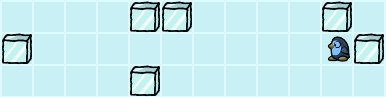
\includegraphics[width=7cm]{img/slide1}

    \vspace{0.5cm}
    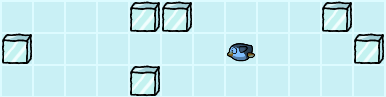
\includegraphics[width=7cm]{img/slide2}

    \vspace{0.5cm}
    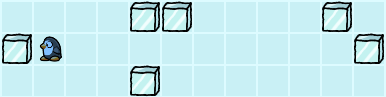
\includegraphics[width=7cm]{img/slide3}

    \caption*{Un agent qui glisse vers l'ouest.}
\end{figure}

\newpage
\paragraph{Pousser}\label{pousser}

Il est possible de pousser un autre agent si ce dernier est sur une case
adjacente à l'un de vos propres agents. Le pousser dans une direction le
fait glisser jusqu'à ce qu'il rencontre un obstacle. Pousser un agent
coûte 5 points d'action.

\begin{figure}[!h]
    \centering
    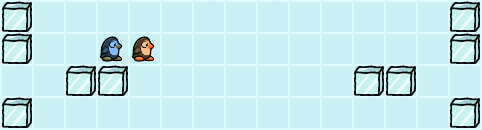
\includegraphics[width=7cm]{img/push1}

    \vspace{0.5cm}
    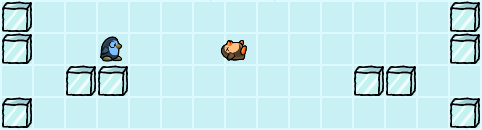
\includegraphics[width=7cm]{img/push2}

    \vspace{0.5cm}
    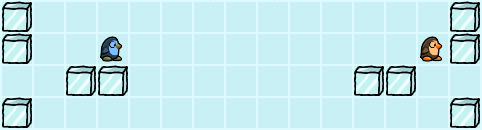
\includegraphics[width=7cm]{img/push3}

    \caption*{L'agent bleu pousse l'agent rouge.}
\end{figure}

À nouveau, les aliens font tout leur possible pour esquiver les agents,
vous ne pouvez donc pas les pousser (ce n'est pas pour rien qu'il faut 3
tours pour les capturer !).

\paragraph{Débug}\label{duxe9bug}

Pour vous permettre de débugger votre intelligence artificielle, il est
possible de placer des drapeaux de débug de trois couleurs différentes
sur la carte que vous pourrez ainsi voir dans l'interface de la
simulation. Cette action ne coûte aucun point d'action.

\begin{figure}[!h]
    \centering
    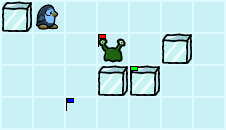
\includegraphics[width=5cm]{img/debug_flags}
    \caption*{Drapeaux de débug.}
\end{figure}

\subsubsection{Score}\label{score}

Chaque alien capturé vous rapporte un certain nombre de points en
fonction de l'alien, selon son espèce, le danger brut qu'il représente,
et ses opinions politiques. La recrue ayant accumulé le plus de points à
la fin de la partie rejoindra les rangs des Prologin in Black pour
lutter contre les invasions intergalactiques.

\subsubsection{Format de la carte}\label{format-de-la-carte}

La carte de l'iceberg est représentée dans un fichier texte qui suit le
format suivant :

\begin{verbatim}
iceberg ASCII
positions depart agents joueur 1
positions depart agents joueur 2
description aliens
\end{verbatim}

La représentation ASCII de l'iceberg est constituée de \texttt{.} pour
une case libre et \texttt{X} pour un mur.

Pour chaque joueur, quatre lignes, une par agent, indiquent la position
de départ d'un agent sous la forme \texttt{ligne\ colonne}.

La description des aliens commence par un nombre sur une seule ligne
indiquant le nombre d'aliens qui envahiront l'iceberg durant la partie.
Chaque ligne précise ensuite les caractéristiques d'un alien :
\texttt{position\_ligne\ position\_colonne\ points\_capture\ tour\_invasion\ duree\_invasion}
